\subsection{Map}
Map is a 2D spatial data type, primarily used for images of the Sun and 
inner heliosphere. It provides a wrapper around a data array (numpy 
ndarray) and gives easy access to standard meta data in the header of the 
image.
The \texttt{Map} datatype provides convenience methods for many functions 
such as, rotation and re-sampling as well as convenience visualisation 
functions.
The design of the map submodule is such that each instrument or 
detector can subclass the parent \texttt{GenericMap} class to implement 
special meta data handling or other data specific functions. Each subclass 
of \texttt{GenericMap} can register with the \texttt{Map} factory class and 
by implementing a method that returns \texttt{True} if the meta data 
matches meta data for that instrument or detector, the \texttt{Map} factory 
will automatically return an instance of the specific \texttt{GenericMap} 
subclass. As of version 0.4 SunPy has \texttt{Map} specialisations for the 
following instruments: \textit{IRIS} SJI frames, \textit{SDO/AIA} and 
\textit{HMI}, \textit{SOHO/EIT} and 	\textit{LASCO}, 
\textit{STEREO/EUVI} 	and \textit{COR}, \textit{YOHKOH/SXT}, 
\textit{RHESSI}, \textit{PROBA2/SWAP} and\textit{HINODE/XRT}.

\begin{listing}[h]
\begin{minted}{pycon}

>>> import sunpy.map

>>> aiamap = sunpy.map.Map('aia_file.fits')
>>> aia
SunPy AIAMap
---------
Observatory: SDO
Instrument:  AIA_3
Detector:    AIA
Measurement: 171
Obs Date:    2011-03-19T10:54:00.34
dt:          1.999601
Dimension:   [1024, 1024]
[dx, dy] =   [2.400000, 2.400000]

array([[ 0.3125, -0.0625, -0.125 , ...,  0.625 , -0.625 ,  0.    ],
       [ 1.    ,  0.1875, -0.8125, ...,  0.625 , -0.625 ,  0.    ],
       [-1.1875,  0.375 , -0.5   , ..., -0.125 , -0.625 , -1.1875],
       ..., 
       [-0.625 ,  0.0625, -0.3125, ...,  0.125 ,  0.125 ,  0.125 ],
       [ 0.5625,  0.0625,  0.5625, ..., -0.0625, -0.0625,  0.    ],
       [ 0.5   , -0.125 ,  0.4375, ...,  0.6875,  0.6875,  0.6875]])

\end{minted}
\caption{Example of printing information about a map at a Python interactive 
prompt.}
\label{code:aia_2}
\end{listing}

\begin{listing}[h]
\begin{minted}{python}

import sunpy.map

aiamap = sunpy.map.Map('aia_file.fits')
aia.peek()
\end{minted}
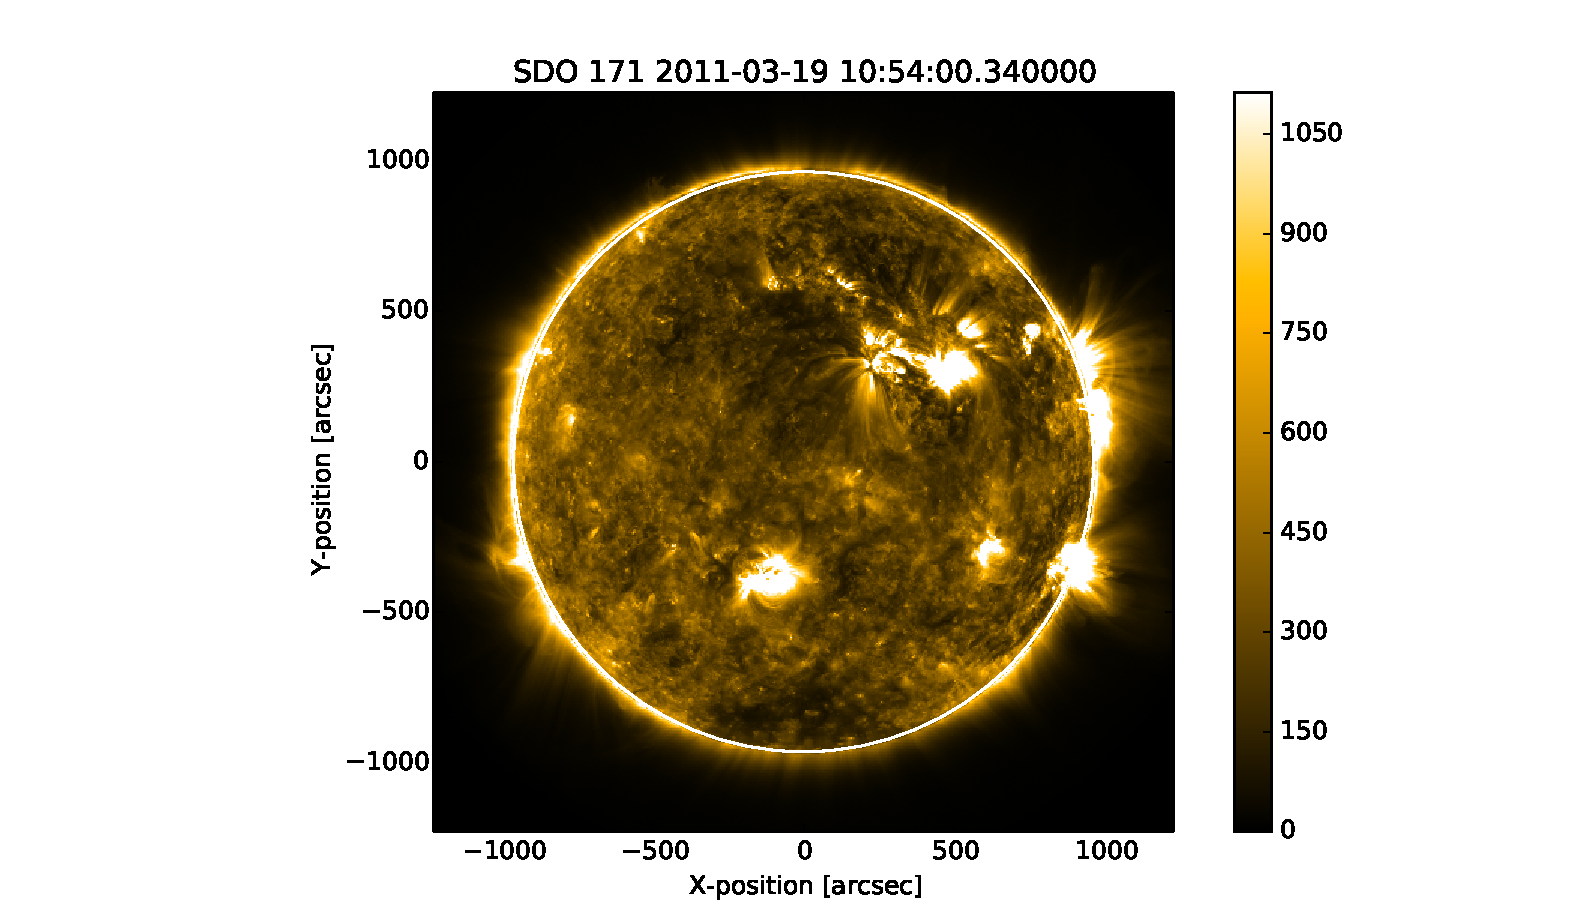
\includegraphics[width=0.8\columnwidth]{aia_map_example}
\caption{Demonstration of the \textit{AIA} map quick view plotting method.}
\label{code:aia_1}
\end{listing}

As can been seen in Listing \ref{code:aia_1} \& \ref{code:aia_2} the map 
datatype parses header information for many purposes including visualisation on 
correct physical axes and limb plotting as well as making this information 
easily available to the user.

As well as providing the base classes the map submodule provides two 
collection classes, \texttt{CompositeMap} and \texttt{MapCube}, for 
temporally and spatially aligned data respectively. \texttt{MapCube} 
provides methods for animation of its series of \texttt{Map} objects. 
\texttt{CompositeMap} provides methods for overlaying spatially aligned 
data, with support for visualisation of images and contour lines overlaid 
upon each other.

\begin{listing}[h]
\begin{minted}{python}
import matplotlib.pyplot as plt
import sunpy.map

#Create a composite map from two files
compmap = sunpy.map.Map('aia_1600_image.fits', 'RHESSI_image.fits', 
composite=True)

#Set the RHESSI image (index 1) to have contour levels and a red colour map.
compmap.set_levels(1,range(0,50,5),percent=True)
compmap.set_colors(1,'Reds_r')

#Plot the result and crop
ax = plt.subplot()
compmap.plot()
ax.axis([200,600,-600,-200])
\end{minted}
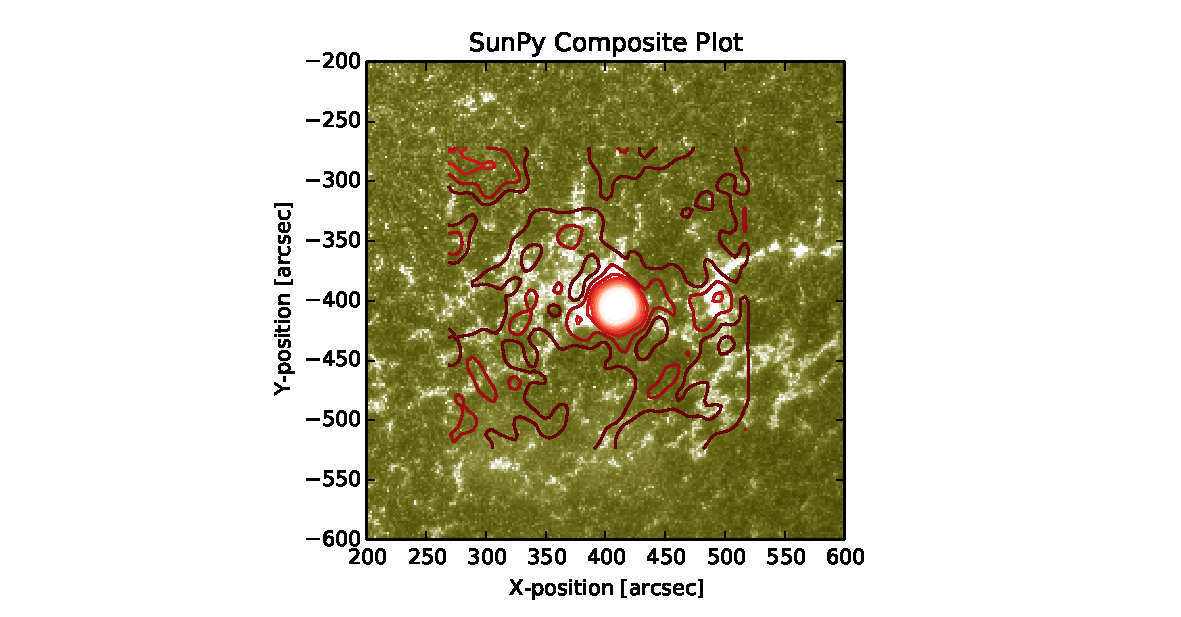
\includegraphics[width=0.8\columnwidth]{comp_map_example}
\caption{Example demonstrating a CompositeMap plot, using contours and how 
SunPy integrates with matplotlib's pyplot functional interface.}
\label{code:compmap_1}
\end{listing}

\begin{listing}[h]
\begin{minted}{python}
import sunpy.map

compmap = sunpy.map.Map('aia_lev1_171a_2014_01*fits', cube=True)
compmap.peek()
\end{minted}
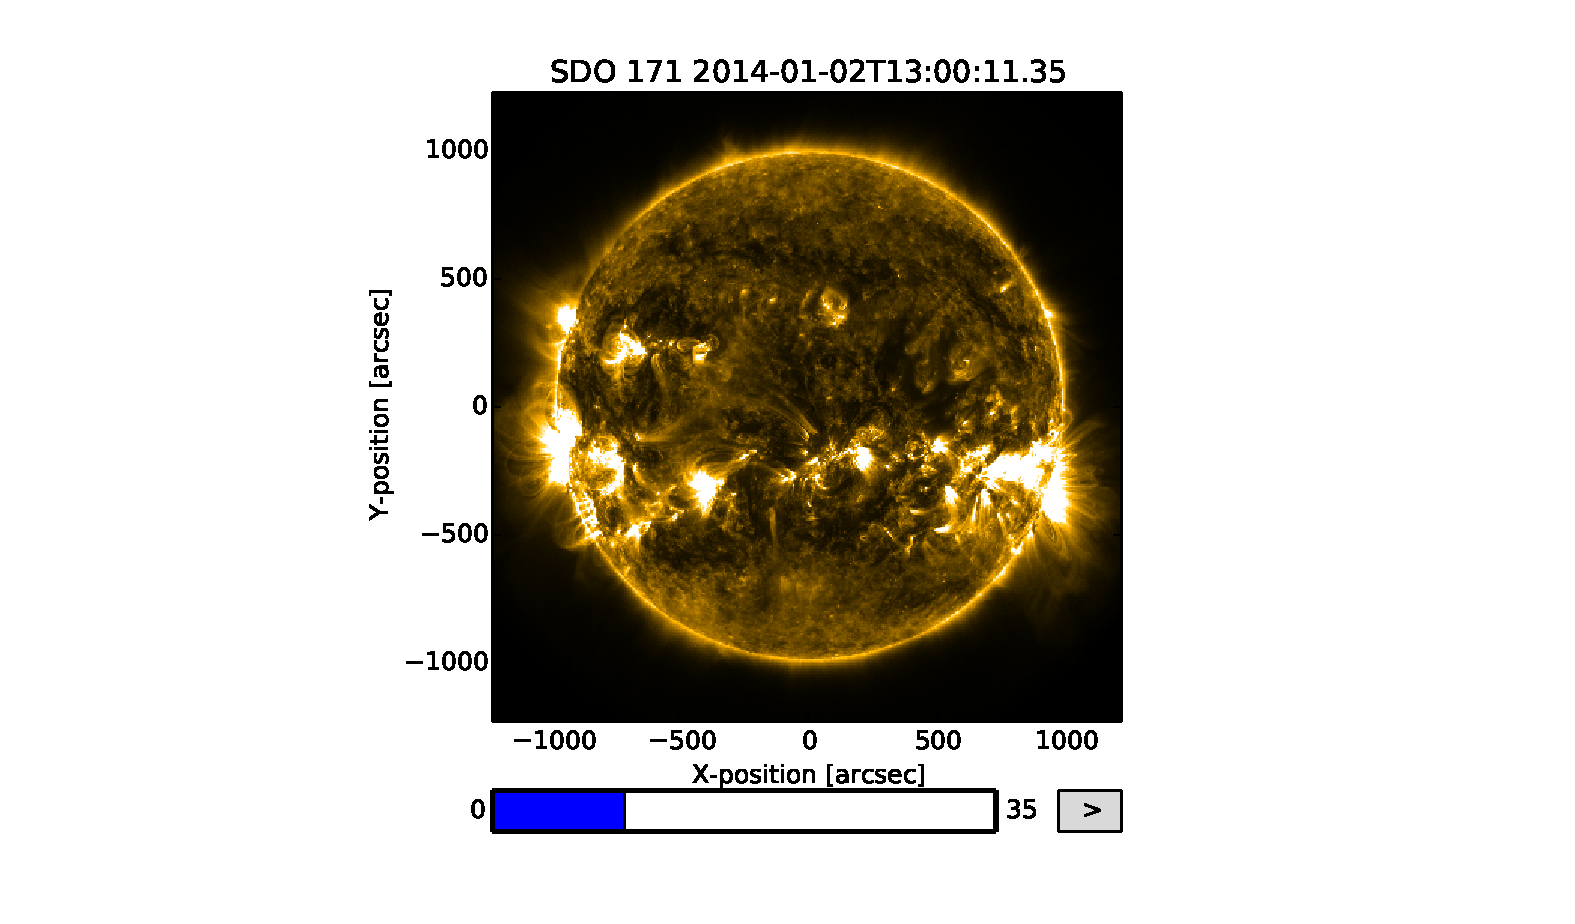
\includegraphics[width=0.8\columnwidth]{aia_cube_controls}
\caption{An example showing creation of a MapCube from a glob file search. The 
resultant plot makes use of matplotlib's interactive widgets to allow scrolling 
through the MapCube.}
\label{code:mapcube_1}
\end{listing}

\begin{listing}[h]
\begin{minted}{python}
import sunpy.map
from matplotlib import animation

mapc = sunpy.map.Map('aia_lev1_171a_2014_01*fits', cube=True)
anim = mapc.plot()
Writer = animation.writers['ffmpeg']
writer = Writer(fps=10, metadata=dict(artist='SunPy'), bitrate=1800)
anim.save('aia_cube.ogv')
\end{minted}
\caption{Example showing how to save a video animation from a MapCube, using 
matplotlib's animation framework.}
\label{code:mapcube_2}
\end{listing}